\section*{Epsilon dynamic}
Note that we can rewrite $\theta(t,s)$ from \ref{eq:theta_ts} by transforming $\eps$ itself in a variable of time:
\begin{equation*}
  \theta(t,s)=\xi(0,t,\eps_s;\theta(0))~~ \text{ where }~~ 
  \eps_s(t)= \mathbbm{1}_{[0,s]}(t)\ .
\end{equation*}
From this formula, a natural question arises: is a step function really the best choice for $\eps(t)$?

To reply, we first need to analyse the dynamics in the very simple case of linear regression with squared loss to see if we can get any insight.\\
With this goal in mind, let's rewrite explicitly \ref{eq:GF} in this specific case (I will use the same notation as the IF vs Leverage part):
\begin{equation}\label{eq:LRGF}\tag{LRGF}
  \begin{cases}
    \frac{d}{d\,t}\theta(t,1) = -\nabla \frac12(X\theta-y)^2=-X^\top X\theta+X^\top y \\
    \theta(0)=\theta_0
  \end{cases}.
\end{equation}
This is a linear ODE, so, when $H$ is invertible, we can find an explicit solution, which reads:
\begin{equation}\label{eq:sol_theta}
  \theta(t,1)=e^{-H t} \theta_0 +(\mathrm{Id}_d-e^{-H t})H^{-1}X^\top y .
\end{equation}

\begin{lemma}
  The system \ref{eq:LRGF} has a unique asymptotically stable equilibrium point:
  \begin{equation*}
    \theta^\star=(X^\top X)^\dagger X^\top y + (\mathrm{Id}_d - X^\top (X X^\top)^\dagger X)\theta_0 ,
  \end{equation*}
  where $A^\dagger$ denotes the Moore-Penrose pseudo-inverse.
  In particular, when $X^\top X$ is invertible, we get:
  $$\theta^\star=\lim_{t\to\infty}\theta(t,1)=(X^\top X)^{-1} X^\top y =\hat\theta_{\mathrm{LS}}.$$
\end{lemma}

\begin{proof}
  The case of $H$ invertible can be proven by looking at the explicit solution stated above: for $t\to\infty$, it yelds: $\theta^\star=H^{-1}X^\top y=:\hat\theta_{\mathrm{LS}}$.
  When $\mathrm{rnk} H=r<d$, let us begin by observing that since $H=X^\top X$, $H$ is diagonalizable, i.e., there exists $Q$ orthogonal matrix such that $H=Q^\top D Q$.
  Therefore, up to permutation matrices, we can rewrite $D$ as diag$(d_1,\dots,d_r,0,\dots,0)$ where $d_1,\dots,d_r\neq0$ and we have $d-r$ zero entries.
  By the definition of the matrix exponential, it holds true that $e^{-Ht}=Q^\top e^{-Dt} Q$ and $e^{Dt}=\mathrm{diag}(e^{d_1 t},\dots,e^{d_r t},1,\dots,1)$.
  For this reason, we can consider the two invariant subspaces $\mathrm{ran}H\oplus\mathrm{ker}H$ and study the dynamic in these two sets.
  \begin{itemize}
    \item In $\mathrm{ker}H$, applying the formula \ref{eq:sol_theta} we get $\theta(t,1)=\pi_{\mathrm{ker}H}\theta_0$;
    \item In $\mathrm{ran}H$, the same formula, if we call $\tilde H=H\vert_{\mathrm{ran}H}$, yields $\theta(t,1)=e^{-\tilde H t} \pi_{\mathrm{ran}H}\theta_0 +(\mathrm{Id}_d-e^{-\tilde H t})\tilde H^{-1}\tilde X^\top \pi_{\mathrm{ran}H}y$.
  \end{itemize}
  To conclude, observe that $\mathrm{ker}H=\mathrm{ker}X$ and $\mathrm{ran}H=\mathrm{ran}X^\top$.
  Therefore, $\pi_{\mathrm{ker}H} = \pi_{(\mathrm{ran}X^\top)^\bot} = I-X^\top (X X^\top)^\dagger X$ (note that here the M-P pseudoinverse pops up naturally from the request of $\pi^2=\pi$) and the projections in the second case are not needed.
  The thesis is achieved by glueing together the results in the two subspaces.
\end{proof}

In order to extend this to the case of every other $\eps\in(0,1)$ 
\footnote{for $\eps=0$ consider for simplicity $X',y'$ obtained by removing the target datapoint, otherwise we can integrate that case in the general one using the Moore-Penrose pseudoinverse}, 
consider \\$y^j_\eps = (y_1,\dots,\eps y_j,\dots,y_n)$ and similarly $X^j_\eps$ and $H^j_\eps=(X^j_\eps)^\top X^j_\eps$.
Solving \eqref{eq:LRGF} with the above quantities defines:
\begin{equation}\label{eq:eq2}
  \theta(t,\eps)= e^{-H^j_\eps t} \theta_0 +(\mathrm{Id}_d-e^{-H^j_\eps t})\hat\theta_{-j}(\eps) .
\end{equation}
With $s,T$ fixed, what we want to study is what is the "fastest route" to $\theta^\star_{-j}$ when we change $\eps_s(t)$.
In other words, we are trying to solve:
\begin{equation}\label{eq:obs_meas}
  \min_{\eps\in E_s}\mathcal{E}(\eps)\quad \text{where}\quad \mathcal{E}(\eps)=\frac12\|\xi(0,T,\eps;\theta(0))-\theta^\star_{-j}\|_\Theta^2
\end{equation}
for $E_s=\{f\in[0,1]^{[0,+\infty]} \mid f(t)=1~\forall t\leq s \wedge f(t)=0 ~\forall t\geq T\}$.

\qst Shall we consider instead $\mathcal{E}(\eps)=\frac12\|\xi(0,T,\eps;\theta(0))-\xi(0,T,0;\theta(0))\|_\Theta^2$ ?

Computed on our baseline (i.e., $\eps_s(t)=\mathbbm{1}_{[0,s]}(t)$), this quantity is:
\begin{equation*}
  \mathcal{E}(\eps_s)=\frac12\|e^{-H_{-j}(T-s)} (e^{-H s} \theta_0 +(\mathrm{Id}_d-e^{-H s})\theta^\star-\theta^\star_{-j}) \|^2.
\end{equation*}
In fact, applying \ref{eq:eq2} for $\eps=1$ and $T=s$ yields the initial condition for the IVP with $\eps=0$, which reads:
\begin{equation*}
  \begin{cases}
    \dot \theta(t,\eps(t)) = -\sum_{i\neq j} x_i(x_i^\top\theta-y_i) \\
    \theta(0) = e^{-H^j_1 t} \theta_0 +(\mathrm{Id}_d-e^{-H^j_1 t})\hat\theta_{-j}(1)
  \end{cases}.
\end{equation*}
Recall that $H^j_1=H$ and $\hat\theta_{-j}(1)$. At this point, using again \ref{eq:eq2} for $\eps=0$ and substituting in the definition of $\mathcal{E}(\eps)$ gives the equality.

\begin{center}
  \textbf{Can we do any better?}
\end{center} 

Unfortunately, as soon as we add the time dependancy of $\eps$ in the equation:
\begin{equation}\label{eq:eps_t}
  \begin{cases}
    \dot \theta(t,\eps(t)) = -\sum_{i\neq j} x_i(x_i^\top\theta-y_i) - \eps(t)x_j(x_j^\top\theta-y_j) \\
    \theta(0) = \theta_0
  \end{cases} ,
\end{equation}
we cannot obtain a closed form solution anymore. In fact, even if we rewrite the first line as:
\begin{equation*}
  \begin{aligned}
    \dot \theta(t,\eps(t)) &= a(t)\theta(t) + b(t), \text{ where } \\
    a(t) &= -\sum_{i\neq j}x_ix_i^\top - \eps(t)x_jx_j^\top \\
    b(t) &= \sum_{i\neq j}x_iy_i + \eps(t)x_jy_j
  \end{aligned}
\end{equation*}
and use the method of the Wronskian with the variation of constants, that does not yield a closed-form solution in the general case\footnote{This method requires $\eps\in C^1$ because to apply the Wronskian we need to take another derivative in the homogeneous equation and consider $\ddot\theta-\dot\theta a(t) - \theta \dot a(t)$.}.\\
Let's see what happens instead for simpler cases doing computations by hand. In the following, consider $s>0$ fixed.

\paragraph{Step functions} Is $\mathbbm{1}_{[0,s]}$ the best step function we can choose in $E_s$?

\begin{lemma}\label{le:step_eps}
  Assume $H=\mathrm{Id_d}$. 
  Given $0\le s < T$, the $\tau$ that minimizes $\mathcal{E}(\eps_\tau)$ in $\{\eps_\tau=\mathbbm{1}_{[0,\tau]} \mid \tau\in[s,T]\}$ is $\eps_s$.
\end{lemma}

\begin{proof}
Starting from the assumption that $H=\mathrm{Id}_d$, we can prove that both $H_{-j}$ and $(H_{-j}-\mathrm{Id}_d)$ are projections, i.e., they have the property that $P^2=P$.
In fact, $H=\mathrm{Id}_d$ iff $X$ is orthogonal. Thus (call $X_{-j}=(I-\hat e_j \hat e_j^\top)X$):
\begin{equation*}
  H_{-j} = X_{-j}^\top X_{-j} = X^\top(I-\hat e_j \hat e_j^\top)^\top(I-\hat e_j \hat e_j^\top)X ,
\end{equation*}
and, since $X X^\top = \mathrm{Id}_d$ and $(I-\hat e_j  \hat e_j^\top)$ is a projection:
\begin{equation*}
  H_{-j}^2 = X^\top(I-\hat e_j \hat e_j^\top)^\top(I-\hat e_j \hat e_j^\top)X X^\top(I-\hat e_j \hat e_j^\top)^\top(I-\hat e_j \hat e_j^\top)X = X^\top (I-\hat e_j \hat e_j^\top) X = H_{-j} .
\end{equation*}
Moreover, it holds that $H_{-j}=\mathrm{Id}_d- v v^\top$ where $v=X^\top e_j = x_j$.
Using the fact that for a projection $P$ holds $e^{a P}=\mathrm{Id_d}+(e^a-1)P$, we can then rewrite $\mathcal{E}(\eps_\tau)$ as:

\begin{equation*}
  \begin{aligned}
    \mathcal{E}(\eps_\tau) &= \frac12\|e^{-(T-\tau)H_{-j}} (e^{-\tau} \theta_0 +(\mathrm{Id}_d-e^{-\tau})\theta^\star-\theta^\star_{-j}) \|^2 \\
    &= \frac12 \|\left(\mathrm{Id}_d + (e^{-(T-\tau)}-1) H_{-j} \right) (e^{-\tau} \theta_0 +(\mathrm{Id}_d-e^{-\tau})\theta^\star-\theta^\star_{-j})\|^2 .
  \end{aligned}
\end{equation*}

To find the optimal $\tau\in [s,T)$, let's compute the derivative in $\tau$ of the previous quantity and study when it is equal to $0$.\\
Recall that $\|x\|^2=\langle x,x \rangle$. 
Thus, if we call 
\begin{equation*}
  g(\tau) = \left(\mathrm{Id}_d + (e^{-(T-\tau)}-1) H_{-j} \right) (e^{-\tau} \theta_0 +(\mathrm{Id}_d-e^{-\tau})\theta^\star-\theta^\star_{-j}),
\end{equation*}
we get that $\frac{d}{d\,t}\mathcal{E}(\eps_\tau)= \langle g(\tau), g'(\tau) \rangle$.
First, let's compute $g'(\tau)$:
\begin{equation*}
  \begin{aligned}
    \frac{d}{d\,\tau}g(\tau) &= e^{-(T-\tau)}H_{-j} (e^{-\tau} \theta_0 +(\mathrm{Id}_d-e^{-\tau})\theta^\star-\theta^\star_{-j}) + \\
    & + \left(\mathrm{Id}_d + (e^{-(T-\tau)}-1) H_{-j} \right)(-e^{-\tau} \theta_0 +e^{-\tau}\theta^\star) =\\
    & = e^{-(T-\tau)} H_{-j}(\theta^\star -\theta^\star_{-j}) +\left(\mathrm{Id}_d - H_{-j} \right)(-e^{-\tau} \theta_0 +e^{-\tau}\theta^\star).
    \end{aligned}
\end{equation*}
Consequently, differentiating $\mathcal{E}$, yields:
\begin{equation*}
  \begin{aligned}
    \frac{d}{d\,\tau}\mathcal{E}(\eps_\tau)
    & = \langle g'(\tau), g(\tau) \rangle \\[0.2cm]
    & = \Big\langle
    e^{-(T-\tau)} H_{-j}(\theta^\star-\theta^\star_{-j})
    + (I_d-H_{-j})(-e^{-\tau}\theta_0 + e^{-\tau}\theta^\star), \,
    g(\tau)
    \Big\rangle \\[0.2cm]
    & = e^{-(T-\tau)}
    \big\langle H_{-j}(\theta^\star-\theta^\star_{-j}), g(\tau)\big\rangle
    + \big\langle (I_d-H_{-j})(-e^{-\tau}\theta_0 + e^{-\tau}\theta^\star),
    g(\tau)\big\rangle \\[0.2cm]
    & = e^{-(T-\tau)}
    \big\langle H_{-j}(\theta^\star-\theta^\star_{-j}),
    H_{-j} g(\tau)\big\rangle
    + \big\langle (I_d-H_{-j})(-e^{-\tau}\theta_0 + e^{-\tau}\theta^\star),
    (I_d-H_{-j}) g(\tau)\big\rangle \\[0.2cm]
    & = e^{-(T-\tau)}
    \big\langle H_{-j}(\theta^\star-\theta^\star_{-j}),
    e^{-(T-\tau)} H_{-j}(\theta^\star-\theta^\star_{-j})\big\rangle \\[0.2cm]
    &
    + \big\langle (I_d-H_{-j})(-e^{-\tau}\theta_0 + e^{-\tau}\theta^\star),
    e^{-\tau}(I_d-H_{-j})(\theta^\star-\theta_0)\big\rangle \\[0.2cm]
    & = e^{-2(T-\tau)}\|H_{-j}(\theta^\star-\theta^\star_{-j})\|^2
    + e^{-2\tau}\|(I_d-H_{-j})(\theta^\star-\theta_0)\|^2 .
  \end{aligned}
\end{equation*}

The above derivative is always positive unless both norms annihilate, which is a probability zero event if we randomly initialise the starting point.
In such case, $\mathcal{E}(\tau)$ is constant because removing the $j$-th datapoint does not change the learning trajectory.\\
We can thus conclude that the function $\mathcal{E}(\tau)$ attains its minimum on the interval $[s,T]$ on $s$, making $\eps_s$ the best candidate among the step functions.
\end{proof}
\begin{remark}
  If we do not assume $H=\mathrm{I}$, the derivative of $g(\tau)$ has the following form:
  $$\frac{d}{d\,t} g(\tau) = e^{-(T-\tau) H_{-j}}\left( [H_{-j}-H]e^{-\tau H}(\theta_0-\theta^\star) + H_{-j}(\theta^\star - \theta^\star_{-j}) \right),$$
  and, when taking the scalar product, it yields:
  \begin{equation*}
    \begin{aligned}
    \frac{d}{d\,t}\mathcal{E}(\eps_\tau) & = \langle g'(\tau), g(\tau) \rangle \\
    & = \big\langle g'(\tau), e^{-(T-\tau) H_{-j}} (e^{-\tau H} \theta_0 +(\mathrm{Id}_d-e^{- \tau H})\theta^\star-\theta^\star_{-j}) \big\rangle \\
    & = \big\langle [H_{-j}-H]e^{-\tau H}(\theta_0-\theta^\star) , e^{-\tau H}(\theta_0-\theta^\star) \big\rangle_{e^{-(T-\tau) H_{-j}}} \\
    & + \big\langle H_{-j}(\theta^\star - \theta^\star_{-j}), \theta^\star - \theta^\star_{-j} \big\rangle_{e^{-(T-\tau) H_{-j}}} .
  \end{aligned}
  \end{equation*}
  {\color{RoyalBlue}
  Since both $H _{-j}$ and $e^{-(T-\tau) H_{-j}}$ are positive semidefinite, the second term is always positive.
  In fact, we can express it as a Mahalanobis distance between $\theta^\star$ and $\theta^\star_{-j}$, where the metric is given by $X_{-j} e^{-(T-\tau) H_{-j}}$.

  The first term is more delicate. 
  If $H_{-j}$ and $H$ commute, also the first term is a Mahalanobis distance with the associated matrix being $x_j^\top e^{-T H_{-j}+\tau(H_{-j}-H)}$, but with a negative sign, thus it is always negative.
  
  In general, however, $H$ and $H_{-j}$ do not commute. 
  Indeed, we can rewrite $H=\sum_{i=1}^n x_j x_j^\top$ and $H_{-j}=H-x_j x_j^\top$ and observe that the commutator is:
  $$[x_i x_i^\top, x_j x_j^\top]= (x_i^\top x_j) (x_i x_j^\top - x_j x_i^\top).$$
  Thus, $H$ and $H_{-j}$ commute only when $x_i \perp x_j$ or $x_i \parallel x_j$ for each $i \neq j$.
  
  We would still have a chance to get a simple formula if $[[A,B],A]=[[A,B],B]=0$.
  But this is not the case:
  $$[[x_i x_i^\top, x_j x_j^\top], x_i x_i^\top] = 2(x_i^\top x_j) (\|x_i\|^2 (x_i x_j^\top+ x_j x_i^\top) - (x_j^\top x_i)x_i x_i^\top) \neq 0.$$
  }
\end{remark}
Note that usually in practice $n>d$ and both $H$ and $H_{-j}$ are full rank. \\
It can also happen that $H_{-j} = H$, for example when $x_j$ is a linear combination of the other $x_i$'s, but in that case, $\theta^\star_{-j}=\theta^\star$ and the derivative is $0$.

\begin{figure}[hbt]
  \centering
  \includegraphics[width=0.6\linewidth]{5.pdf}
  \caption{Plot representing the training trajectories for $X=\mathrm{Id_2}$, $y=(1,1)$, $\theta_0=(0,0)$ and $j=2$.}
\end{figure}

\paragraph{Linear functions} Consider the class of functions $\eps_{\mathrm{lin}, t_1}(t)$ such that:
\begin{equation*}
  \eps_{\mathrm{lin}, t_1}(t)= \mathbbm{1}_{[0,s]}(t)+\mathbbm{1}_{[s,t_1]}(t)\left(1-\frac{(s-t)}{(s-t_1)}\right).
\end{equation*}
The main problem is that now in \ref{eq:eps_t} from $s$ to $t_1$ we have the following non-autonomous equation:
\begin{equation*}
  \begin{cases}
    \dot \theta(t,\eps(t)) = -\sum_{i\neq j} x_i(x_i^\top\theta-y_i) - \left(1-\frac{(s-t)}{(s-t_1)}\right)x_j(x_j^\top\theta-y_j) \\
    \theta(0) = \xi(0,s,1;\theta_0)
  \end{cases} .
\end{equation*}
To try solve this, let's define $\psi(t)=t$, thus $\dot \psi = 1$. Then, we can the previous equation as a dynamical system:
\begin{equation}
  \begin{cases}
    \dot \theta(t) = \left(-\sum_{i\neq j} x_i x_i^\top \right)\theta(t) + \frac{x_j x_j^\top}{s-t_1} \theta(t) \psi(t) + \left(\sum_{i\neq j}x_i y_i + (1-\frac{s}{(s-t_1)})x_j y_j\right) \\
    \dot \psi(t) = 1
  \end{cases}.
\end{equation}
Note that this system is a special case of an inhomogeneous Lotka-Volterra system and it has no closed form solution.
Unfortunately, I think that even though we can describe qulitatively the solutions, for our purpose we would need quantitative results, which I don't know how to obtain.

\paragraph{General case} 
Since the general statement is clear and from my perspective the optimal solution should be a step function, I would like to try and approach this problem from a more general point of view, hoping to exploit some deeper structure that could avoid us some intricate computation.
My idea is that we can check optimality of $\eps(t)$ by imposing that at each time, the deplacement is maximum towards $\theta^*_{-j}$. 
In this sense, we could consider the global ODE as an uncountable set of ODEs with fixed $\eps$ and, since we know the explicit solution in this case, we can maximize the previous quantity.
My hope is that we always get that optimality is achieved by setting $\eps=0$ for every instance.

Let me give a formalization of the above mentioned procedure (I am not sure about considering an ODE at each $dt$, but if we use Gradient Descent it totally makes sense to consider $T$ different equations).\\
In the gradient descent case, I would consider the quantity:

\begin{equation*}
  (\theta(t+1)-\theta(t))\cdot\frac{\theta^\star_{-j}-\theta(t)}{\|\theta^\star_{-j}-\theta(t)\|} .
\end{equation*}

If we see $(\theta(t+1)-\theta(t))$ as $(\theta(t+\delta)-\theta(t))/\delta$ for $\delta=1$, then taking the limit for $\delta\to0$ yields the derivative.
Therefore, I would like to maximize the quantity:

\begin{equation}\label{eq:eq1}
  \dot\theta(t)\cdot\frac{\theta^\star_{-j}-\theta(t)}{\|\theta^\star_{-j}-\theta(t)\|} .
\end{equation}

In addition, since we want to change $\eps$ at every time, we should also update the initial condition $\theta(0)$ accordingly and then consider $\dot\theta(0)$.\\
Substituting $t=0$ in \ref{eq:eq1} and computing explicitly the derivative of $\theta(t,\eps)$ from \ref{eq:eq2} yields:

\begin{equation*}
  \frac{\langle -H^j_\eps \theta_0 +(\mathrm{Id}_d + H^j_\eps)\hat\theta_{-j}(\eps) , \theta^\star_{-j}-\theta(0)\rangle}{\|\theta^\star_{-j}-\theta(0)\|} = 
  \frac{\langle (\mathrm{Id}_d + H^j_\eps) (\hat\theta_{-j}(\eps)-\theta(0)), \theta^\star_{-j}-\theta(0)\rangle}{\|\theta^\star_{-j}-\theta(0)\|} + \frac{\langle \theta(0), \theta^\star_{-j}-\theta(0)\rangle}{\|\theta^\star_{-j}-\theta(0)\|}.
\end{equation*}

Note that the second term does not depend on $\eps$ (at this step; it depends however on previous steps, since they lead to $\theta_0$).\\
If we choose $\eps = 0$, then $\hat\theta_{-j}(\eps) = \theta^\star_{-j}$. Thus (let's assume $H=\mathrm{Id}$), the previous quantity equates:

\begin{equation*}
  2\|\theta^\star_{-j}-\theta(0)\| - \frac{([\theta^\star_{-j}-\theta(0)]_j)^2}{\|\theta^\star_{-j}-\theta(0)\|} + \frac{\langle \theta(0), \theta^\star_{-j}-\theta(0)\rangle}{\|\theta^\star_{-j}-\theta(0)\|}.
\end{equation*}

However, this may not be the maximum we can get!
Indeed, if $\theta^\star_{-j}-\theta(0)$ is for example a line parallel to $\theta^\star_{-j}-\theta(0)$, choosing a bigger $\eps$ may be better.

\vspace{0.2cm}\noindent
\textbf{Example:} consider $X=(1,1)^\top$, $y=(y_1,y_2)^\top$, $j=1$. In this case, the system \ref{eq:eps_t} becomes:
\begin{equation*}
  \begin{cases}
    \dot \theta = \eps(y_1-\theta)+(y_2-\theta) \\
    \theta(0) = \theta_0 \in \R
  \end{cases}.
\end{equation*}
Here, $\theta^\star_{-1}-\theta(0)$ is aligned with $\theta^\star_{-1}-\theta(0)$ and if we choose $\theta_0=0$, $y_1=2$, $y_2=1$, then the biggest step is actually achieved by $\eps = 1$.
Indeed, $\hat\theta=y_1+y_2$ and $\hat\theta_{-1}=y_2$, since the general solution is $\theta(t)=e^{-(1+\eps)t}+(1-e^{-(1+\eps)t})(\eps y_1+y_2)$.

\paragraph{Numerical experiments}
Let's see if we can get some more insights with numerical experiments:
\begin{figure}[ht]
\centering
\begin{subfigure}{0.30\textwidth}
\centering
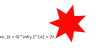
\includegraphics[width=\linewidth]{1.pdf}
\caption*{(a)}
\end{subfigure}
\begin{subfigure}{0.30\textwidth}
\centering
\includegraphics[width=\linewidth]{2.pdf}
\caption*{(b)}
\end{subfigure}

\vspace{0.5em}

\begin{subfigure}{0.30\textwidth}
\centering
\includegraphics[width=\linewidth]{3.pdf}
\caption*{(c)}
\end{subfigure}
\begin{subfigure}{0.30\textwidth}
\centering
\includegraphics[width=\linewidth]{4.pdf}
\caption*{(d)}
\end{subfigure}

\caption{Phase portrait of the numerical integration of the IVP \ref{eq:eps_t} for different $\eps(t)$ and initial conditions $\theta_0$ when $X\in\R^{20\times2}$.
In (a) we can see that changing $\eps$ too late in the training results in way worse results compared to $(b)$, where, if chosen carefully, $\eps>0$ can be faster than LOO. 
However, choosing a different initial condition, as shown in (c), can lead to every $\eps>0$ to be suboptimal. Figure (d) shows that linear decay is slower than stepwise decay.
}
\label{fig:exp_2}
\end{figure}
From the results in Figure \ref{fig:exp_2}, the function $\mathbbm{1}_{[0,s]}$ appears not to be the minimizer for every instance of the problem, as proven in the stepfunction paragraph. 
Moreover, it seems to hold that step functions are better than polynomial decay.
% Another method that may produce some more interesting results is the application of optimal control theory.
% Namely, we can apply the Pontryagin Maximum Principle for linear equations with variable coefficients (cf. \cite{pontryagin_max_princ} Theorem 15 p.184):
% \begin{theorem}[PMP]
%   Consider a system of differential equations of the form:
%   \begin{equation*}
%     \frac{d\,x^i}{d\,t} = \sum_{\nu=1}^{n}a_\nu^i (t) x^\nu + \sum_{\rho=1}^{r} b_\rho(t) u^\rho + f^i(t) \quad i=1,\dots,n~.
%   \end{equation*}
%   Call $A=(a_\nu^i)_{\nu,i=1}^n \in \R^{n \times n}$, $B = (b_\rho)_{\rho=1}^r \in \R^{n \times r}$. 
%   If $A^{\otimes i} B$ are linearly independent for every $i$ and if $A(t),B(t)$ are at least $n$ times differentiable, then
%   there exists a unique solution $u(t)=(u^1,\dots,u^r)\in U$ such that the flow $x(t)$ gets from $x(t_0)=x_0$ to $x(t_1)=x_1$ in minimum time.
%   Moreover, $u$ is piecewise constant and its values are vertices or the polyhedron $U$.
% \end{theorem}
% We can apply this to our case for $x^i=\theta_i$, $u^j=\eps$; it follows that the optimal $\eps$ is piecewise constant and can only take on values $0$ or $1$.\\
% In particular, I think it shouldn't be too difficult to prove that it is constantly $0$, but direct computations may be heavy.\\
% In addition, note that we do not make any assumptions (except sufficient regularity) on $a(t),b(t),f(t)$. Therefore, this theorem is applicable also for the general case with $C^\infty$ activation functions.

% On the negative side, however, this theorem does not solve our problem! In fact, we are not seeking a time-optimal solution (as the time required to get to the optimal point will always be infinite).\\
% We can circumvent this issue by considering a point which is not critical but it's close enough to $\hat\theta$ as an endpoint. 
% At this point, we don't need to consider the problem as in \ref{eq:obs_meas}; instead, we can treat it as a time-minimal problem.

\subsection*{Choice of distance measure}

In the definition of our minimization problem in \ref{eq:obs_meas}, the choice of $\mathcal{E}(\eps)$ was arbitrary.
What is important, is that $\mathcal{E}(\eps)=d(\eps,0)$ for some $d:E_s\times [0,1]^{[0,+\infty]} \to \R$ distance in the metric space of functions from $\R_+$ to $[0,1]$.
Let's discuss more in detail some choices for $d(\eps)=d(\eps,0)$ and what does it mean to implement them.
\begin{itemize}
  \item $d(\eps) = \frac12 \|\xi(0,T,\eps;\theta(0))-\xi(0,+\infty,0;\theta(0))\|^2_\Theta$ : 
  minimizing this quantity is equi\-valent to minimize $\|\frac{1}{2}\|\xi(0,T,\eps;\theta(0))-\theta^\star_{-j}\|_\Theta$, which is the distance in the space of parameters between the optimal
  parameter for the LOO retraining and the parameter obtained at time $T$ of training with the weight switch $\eps\in E_s$.
  In simpler words: "we take the most out of your data before completely forgetting about it".
  
  \item $d(\eps) = \frac12 \|\xi(0,T,\eps;\theta(0))-\xi(0,T,0;\theta(0))\|^2_\Theta$ : 
  in this case, we are comparing the trajectory for the LOO with the one obtained changing weights with $\eps(t)$ at the same final time $T$.
  Simply said: "at the moment of removing your data, we learnt the same as if we hadn't been using your data from the start".
  
  \item $d(\eps) = \frac12 \min_{t>0}\|\xi(0,T,\eps;\theta(0))-\xi(0,t,0;\theta(0))\|^2_\Theta$ : 
  this choice is more difficult to implement, as it is a double minimization problem. 
  In fact, we are trying to find the final point of trajectory obtained by training with $\eps(t)$ which is closest to the orbit of parameters trained with LOO.
  The advantage compared to the first option is that we are more likely to be close the LOO trajectory; in relation with the second distance, this one ensures a better usage of the informations, as we can end up farther. 
  In other words: "We used your data to speed up the training we would have achieved without your information".  
\end{itemize} 
As far as proofs are concerned, in the stepwise case, Lemma \ref{le:step_eps} works for all 3 of the above cases, since we never utilize any property of $\theta^\star_{-j}$.

\section*{What is the problem?}
We are given a training set $D=\{(x_i,y_i)\}_{i=1}^n$ and an index $j\in [n]$ of a data point in the training set. We are also given a learning algorithm $\mathcal{A}(D)$, which, for simplicity, we will assume to be gradient flow on the empirical risk.
Our goal is to find a modification function $\mathcal{M}$ for the algorithm $\mathcal{A}$ that will approximate the effect of retraining the model from scratch on $D\setminus{(x_j,y_j)}$.
To do so, we want to choose $\eps(t)$ from \ref{eq:eps_t} among a class of functions $E_s$ that will allow us to forget the $j$-th data point as much as possible before time $T$, while achieving a good performance as a predictor.

For this problem to be well posed, we first need a proper definition for ``forgetting a data point".
In the literature, I could find two different definitions for this concept, which are the following:
\begin{itemize}
  \item \emph{Certified Removal} \cite{guo_certified_2023}: given $\alpha>0$, we say that $\mathcal{M}$ is an $\alpha$-certified removal algorithm if:
  \begin{equation*}
    e^{-\alpha} \leq \frac{\P(\mathcal{M}(\mathcal{A}(D),j)\in S)}{\P(\mathcal{A}(D\setminus\{(x_j,y_j)\})\in S)} \leq e^{\alpha} \quad \forall S\subseteq\Theta.
  \end{equation*}
  \item Same distribution \cite{papernot_unlearning_2020}: let $\mathbb{D}_\mathcal{M}$ denote the distribution of models learned using mechanism $\mathcal{M}$ on D trying to unlearn the $j$-th data point.
   Let $\mathbb{D}_\text{real}$ be the distribution of models learned using $\mathcal{A}$ on $D\setminus\{(x_j,y_j)\}$.
   $\mathcal{M}$ is a good unlearning algorithm if $\mathbb{D}_\mathcal{M}=\mathbb{D}_\text{real}$.
   This definition is equivalent to $0$-CR.
\end{itemize}
However, I don't think either of these definitions is what I am looking for.
In fact, I am convinced that as long as $\mathcal{M}(\mathcal{A}(D),j)$ ends in a point that can be reached by $\mathcal{A}(D\setminus\{(x_j,y_j)\})$, then we can say that $\mathcal{M}$ is a good unlearning algorithm.
The reason for this is that the gradients only depend on the spatial position of $\theta$ and not on time. 
Thus, I'm expecting that there is no way to extract information about the forgotten data point from a gradient that can be computed without using such data. \\
The main advantage of this definition is that if $\mathcal{M}$ was the oracle algorithm, it would be considered a good unlearning algorithm, whereas for the previous definitions it is not.

Written more formally, I would like to say that $\mathcal{M}$ is a good unlearning algorithm if $\P(\mathcal{M}(\mathcal{A}(D),j)\in B_\beta(\mathcal{A}(D\setminus\{(x_j,y_j)\})))=1$ for any $\beta>0$,
where $B_\beta(\mathcal{A}(D\setminus\{(x_j,y_j)\}))$ is the ball of radius $\beta$ around $\mathcal{A}(D\setminus\{(x_j,y_j)\})$.
Note that if the algorithm $\mathcal{A}$ starts from a random initial condition, then $\mathcal{A}(D)$ is a random variable.\\
For the sake of clarity, I will rewrite this condition in the notation we have been adopting so far.
\begin{definition*}
    We say that $\eps(t)$ induces a good unlearning algorithm $\mathcal{M}$ if, for each $\theta_0\in\Theta_0\subseteq\Theta$, 
    for each $\beta>0$ there exist (at least) a feasible initial condition $\theta\in\Theta_0$ and $t<T$ such that:
    $$ \xi(0,T,\eps(t);\theta_0)\in B_\beta (\xi(0,t,0;\theta)) .$$
\end{definition*}
{\color{RoyalBlue}
This definition makes sense because by the ``continuous dependency from initial condi\-tions'' theorem, the flux of those two differential equations will stay arbitrarily close from $T$ on. \\
Additionally, this theorem gives us an explicit bound on the distance between the two trajectories after a time $t_1$ from the meeting point, if they have minimum distance $\beta$:
\begin{equation*}
  \|\xi(0,\cdot,0;\xi(0,T,\eps(t);\theta_0)) - \xi(0,\cdot,0;\xi(0,t,0;\theta))\|_{\infty,[0,t_1]} \leq e^{L t_1} \beta,
\end{equation*}
where $L$ is the Lipschitz constant of the $-\nabla_\theta R_j$.

\begin{lemma}
  Call $\tilde{\theta}(s) = \xi(0,s,0;\xi(0,T,\eps(t);\theta_0))$ and $\theta(s) = \xi(0,s,0;\xi(0,t,0;\theta))$.
  Assuming that the data points are normalized, i.e. $\|x_i\|_2=1$ for $i=1,\dots,n$, it holds true that for any $s\in[0,t_1]$:
  \begin{equation*}
    \| \nabla L(\tilde{\theta}(s)) - \nabla L(\theta(s)) \|_2 \leq n e^{L t_1} \beta.
  \end{equation*}
\end{lemma}

\begin{proof}
  Assume $\Theta\subseteq \R^d$ with the Euclidean norm.
  Let's compute the difference between the two gradients:
  \begin{equation*}
    \begin{aligned}
      \| \nabla L(\tilde{\theta}(s)) - \nabla L(\theta(s)) \|_2 &= \| \sum_{i=1}^n x_i (x_i^\top \tilde{\theta}(s) - y_i) - \sum_{i=1}^n x_i (x_i^\top \theta(s) - y_i) \|_2 = \\
      & = \| \sum_{i=1}^n x_i x_i^\top (\tilde{\theta}(s) - \theta(s)) \|_2 \leq \sum_{i=1}^n \|x_i\|_2^2 \|\tilde{\theta}(s) - \theta(s)\|_2 \leq n e^{L t_1} \beta.
    \end{aligned}
  \end{equation*}
\end{proof}

\begin{remark}
  If we can approximate exactly $\theta^\star_{-j}$, then all the definitions are satisfied.
  Name\-ly, in the case of Linear Regression with the squared loss, the Newton method (IF estimation) is exact and therefore it's a good unlearning algorithm.
\end{remark}

Some applications of the influence functions I would eventually like to investigate include:
\begin{itemize}
  \item recognition of informative images in a set;
  \item variation of weights for mislabeled samples (in this case, it is useful to study what is the $\eps(t)$ that minimizes the distance from optimum at the end of the training).
\end{itemize}
}
